\chapter{Introduction}
% 1st sect: GENERAL BACKGROUND: data environments evolve. data stream processing requires being accurate efficiently.
A problem occurring in nearly every application of machine learning is the challenge of handling evolving environments, a problem known as concept drift. Meanwhile, the domain of data stream processing proposes its own set of challenges, the main one being the ability of providing accurate predictions at any time despite large volumes of data and constrained time and memory resources. The combination of these two problems, the need to adapt to evolving data while meeting the systems requirements, is complex, but common.

% there are lots of solutions to this so requirements are needed to select from them
Multitudes of approaches have been proposed as a solution to the problem of handling concept drift efficiently in stream processing systems, each with their own set of strengths. Therefore, to be able to compare the applicability of these solutions, a set of requirements should be used as a starting point. A case study is presented for this purpose, and the solution is searched for given the set of identified assumptions and requirements. 

% the context intro
The thesis at hand uses as context an on-going research project, VesselAI, aiming for applying novel machine learning to the domain of maritime. The domain in question is characteristic in the especially large volume of incoming sensor data and the slowness of vessel traffic in comparison. Additional context specifics include low-quality and heterogeneousness of data, the complexity and novelty of the deep learning models used, and the delayedness of model feedback. 

% goal
The goal of this analysis is, given the project context, to find the most optimal approach for maintaining model accuracy. In other words, from the challenges identified in the VesselAI state-of-the-art analysis \cite{D1.1}, the problem tackled is `ML model retraining is computationally very heavy: in environments where data evolves, it is urgent to use architectures that manage ML models in order to adapt to new data/tasks and retrain when necessary'. In addition to the suggested approach of lifelong learning, additional insight is gathered from the research fields of concept drift adaptation, batch learning, and AutoML.  This way literature gap of works addressing the maritime domain and automated model adaptation identified in \cite{D1.1} is addressed.   

% systems perspective
Traditionally, works addressing the problem of concept drift largely focus on how to build a model that is able to adapt to the changing environment. This thesis can, from this perspective, also be seen as a systems approach to concept drift. If a model is taken as given, it is discussed how the system organization would be able to make sure the model stays accurate. This perspective also aims to take into account the insight on best practices from the field of designing big data systems. From the lessons learned there it is especially aimed for a solution that is simple and mature enough to be applied to a real-world scenario.

% 2nd section: RESEARCH Q'S, METHODOLOGY, RESULTS SUMMARY

% outline
% main question
% exact definitions of main question
% sub-questions
% note on methodology (literature based but not systematic, non-empirical)
% results summary

% comment: the sentence on the model is a little vague, tailored means that it is made for the case not just taken from somewhere else. I'm unsure what words to mention on the model here.

% research question
The main research question addressed in this work is the following:

\begin{center}
    Given the domain context and the models used, how to organize a workflow for efficient updating of the models in order to meet the demands posed by the use case?
\end{center}

As further elaboration, by updating the model it is meant that the model parameters are changed. By efficient we mean efficiency relative to the data volume, not relative to computing resources. This means that an average high performance cluster is assumed and the target is to be able to utilise that to be able to handle as much data in as little time as possible. The domain context used is the maritime domain, and the model used is assumed to be a deep learning model operating in batch mode.

The secondary research questions considered as implications of the primary one are the following:

\begin{itemize}
    \item Is it possible to organize retraining effectively enough to handle incoming data, or does the model itself need to be adaptable?
    \item How much human intervention is required for maintaining the updating schemes; what are the possibilities of automating these workflows?
\end{itemize}

% add paragraph on results here later...

As a note on methodology, the investigation in its entirety is based on literature. Conducting a systematic literature review would be beyond the scope of this thesis, so only material directly relevant regarding the specific set of requirements is taken into account. Testing the various approaches in practice is also beyond scope; the empirical investigation of these findings is left to future works. This limits both the set of options considered to those already used in the problem domain and the evaluation to analyzig the thoroughness of existing evidence in literature.

% 3rd section: CHAPTER ROLES
% if the result is so that multiple can be good then change chap 4 description to state that the systems applying the max two best seeming options are presented.

The rest of this thesis is organized as follows:

Chapter 2 presents the necessary background knowledge to the reader: an overview of the general organization of a big data system, definitions in the field of machine learning model updating, and an introduction to the maritime domain. Chapter 3 analyzes the various model updating approaches presented previously and discusses which approaches would be most useful given the context of the case. Then, ways of automating the optimal-seeming approaches are shortly discussed. Chapter 4 synthesizes the findings above and presents an abstract overview of the system that would apply the optimal updating workflow. In addition it is discussed how certain these findings are given the quality and thoroughness of the literature used. The thesis is concluded with discussion on the applicability of the results achieved to similar problems from different domains.

\chapter{Overview on large-scale machine\\ learning systems for maritime}

% in case a neural networks introduction is needed: \cite{ben-nun_demystifying_2019} sect 4.1 has a good description

% ingressi: mitä aiot rakentaa luvussa, mikä tulee esille, miksi se on tärkeää, mihin tällä kokonaisuudella pyritään

The general task of big data systems is that they should be able to handle vast amounts of data and from that be able to provide predictions in a timely manner. To position our problem of model maintenance in this larger domain, this chapter provides an introduction to the necessary background. First, the entire big data pipeline is presented on an abstract level, alongside best practices of systems design. Then, to clarify the terminology, machine learning approaches for efficient model updates are defined. Lastly, the requirements of the case used to compare the maintenance approaches are derived from the application domain description.

\section{Introduction to big data systems}

% MLOps is a term that should be used / mentioned somewhere

% current main concern for this sect: I state out a lot of facts without giving a reference -> the fine line between common knowledge and what needs backing...

% add here: this system presented is a ml one, some notes added specifically on the usage of neural networks in these systems

\subsection{The high-level components}

% add here: eg DATE n kung fu papers (1st & 2nd from lucy) state that in ML systems distribution is of high importance. add to model training part
%kungfu: stochastic gradient descent (SGD) algorithm is common, give that as an example maybe?

% the automl survey can be ref'd here. add here a note on what automl + possibly mlops is.

% maybe add: model development. in neural networks neural architecture search is a major computational problem that has a lot of automl research attention. however, this operation is only needed when the model is first developed, not during updates, so its optimization is not considered

The steps that most large-scale machine learning systems compose of are displayed in the following figure: 

% how do I properly cite the google cloud developer guide?
% the figure is too small... -> not very readable
\begin{figure}[ht]
%\begin{figure}[tbh] t= top, b = bottom, h=here
\ \newline
\begin{center}
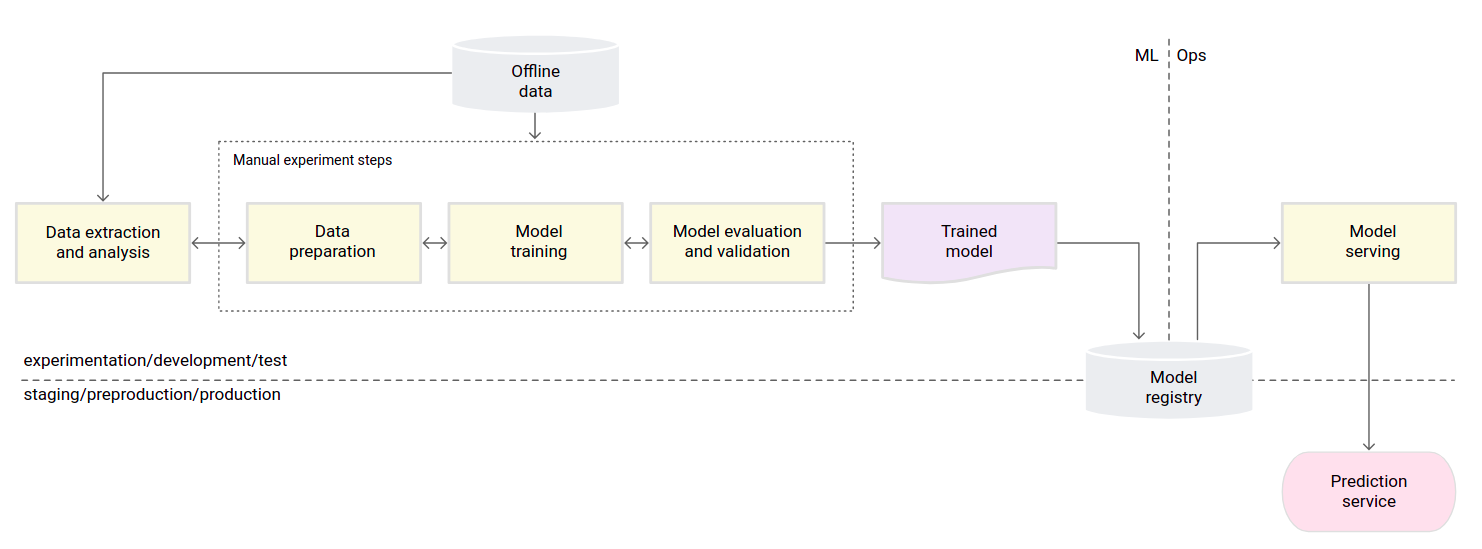
\includegraphics[width=0.9\textwidth]{simplegoogle.png}
\caption{Abstract components of a big data analytics system. From Google Developer MLOps guide~\cite{googlemlops}.}
\label{simplepipeline}
\end{center}
\end{figure}


While the steps above represent a coarse abstraction, hiding away feedback loops and the multitudes of ways each part can be implemented, most contemporary big data systems implement all of the following steps:

\textbf{Data extraction}: this component is responsible for handling the incoming data. Usual forms of data are either web logs, coming in from a server, or IoT data, coming in from sensors that are often geographically distant from the data ingesting component.
% that data is usually web logs or sensor requires a reference?

In big data systems incoming data is represented either as batches, meaning chunks of data coming in at certain intervals, or as a stream, meaning that individual data records are coming in constantly. The main advantage of using a batch representation is known to be increased throughput%(find citations here)
, while stream processing allows smaller end-to-end latencies. %(find citations here)
% the usually interpreted as stream or batch needs a ref too?

To mitigate the tradeoff between throughput and latency, a popular solution is called the lambda architecture. This reference architecture has a processing unit for both batch and stream data with the stream component, so-called speed layer, handling requests for the data not yet processed by the batch layer \cite{beatingcap}. While this approach is widely accepted to solve the problem of handling highly voluminous data fast and mitigating human errors by allowing restarting the speed layer any time without losing data \cite{lambdakappa}, the architecture has faced criticism for being redundantly complex and forcing the data ingestion code to be written twice \cite{questioninglambda} \cite{uber} \cite{facebook}. As an alternative, the kappa architecture has been proposed, only composing of either a batch or a stream processor, usually the latter \cite{questioninglambda}. This mitigates duplication, but retains the tradeoff with throughput and latency \cite{lambdakappa}.

\textbf{Data preparation}: This step encompasses the processes of data cleaning, transformation, and feature engineering. Data cleaning refers to operations identifying and removing faulty data, such as values that are missing or are clearly impossible. Data transformation and feature engineering are used interchangeably, both meaning processes that transform data into a format that the models used can process. A popular example in this is the mapping of plain text into word count matrices \cite{dapbook}.

While the data preparation step is often overlooked in literature,
it is a both challenging and crucial part of the system as preprocessing commonly takes up a majority of the total end-to-end latency of a machine learning system \cite{adaptivelearningsystems}. As for systems design, the most relevant decision to make is whether to clean data before it is saved to the data storage, or only when it is  needed for training. The main benefit with the first approach is that data only needs to be cleaned once, while the latter allows processing data for different models in different ways.
% the two approaches and their tradeoffs need a ref...
% the how many % of time preprocessing takes needs a ref... i got one somewhere...

\textbf{Data storage}: Interpreted in the figure as offline data, the data storage is used to save the data that is needed for model training. The most often used storage methods are called data warehouses and columnar databases. Due to the volume of the data, the storage is either cleared often completely or only a small part of the data is archived.
% data archival needs a ref.
% popular ways of implementing data storage too!

\textbf{Model training}: This component is responsible for training the model, which means tuning the model parameters in a way that it fits to the distribution of the incoming data in order to make accurate predictions from data coming in during operation.

The training conducted can be done from scratch, meaning that the same instance of the model has not been trained before, or in cases of using adaptation-capable models, the models can be updated. Details on model updating or retraining are discussed below.

% changes: federated is definitely considered! + add quick intro to SGD=stochastic gradient descent, the goto algo for distributing neural nets
As for infrastructure, training can be conducted in a central or federated manner. Centralized training, often run in a cloud data center, can run either on one machine or distributed across multiple cores by splitting the model or the data to parallelize the training \cite{iotsurvey}. As the amount of data is large, high-performance computing (HPC) clusters and modern general processing units (GPU) are used to reach required latencies \cite{iotsurvey}. Federated approach refers to an internet of things setting where the training is conducted in the edge devices of the IoT network. This aims to solve the issues of moving privacy-sensitive data across the network and being able to adapt to the unique environments of each data source \cite{iotsurvey}. As in the maritime context the data is neither highly private or has differing environments in different sensors, the federated approach is not considered further in this work.

\textbf{Model evaluation and validation}: In this stage the model is tested and adjusted in various ways. For testing, usually various model metrics such as accuracy for classifiers and error statistics for regression tasks are checked \cite{iotsurvey}. These numbers can also be compared against other models, possibly models already in operation \cite{googlemlops}. Also testing different data sets and checking compatibility with the rest of the system is conducted at this stage \cite{googlemlops}.

In addition to testing, models are also optimized for the infrastructure that they are being deployed on. This can include, for example, various performance optimizations, or in case of constrained memory, model compression \cite{iotsurvey}.

\textbf{Model registry}: is a centralized storage for the trained models. 

% need a reference here as well...

\textbf{Model inference}: edge fog cloud here marked in the figure as 'prediction service', this component contains the trained models that are used for answering application requests. These requests can require data statistics, computed with conventional data analytics, or predictions made by machine learning models.

The most important design decision to make for this component in the sensor data scenario is where to deploy the models, in the cloud, a cloudlet or 'fog', or on the edge. Cloud means that the model is deployed in a data center and edge refers to models being deployed in the IoT devices. Fog refers to the in-between solutions: 

OCF is The Open Connectivity Foundation. add below + the proper source

The definition of fog computing is the following, as stated by the the OCF (in \cite{fogsurvey} reference [42]): “Fog computing is a horizontal, system-level architecture that distributes computing, storage, control and networking functions closer to the users along a cloud-to-thing continuum.” (but not only entirely to the edge). Or, put differently by \cite{fogsurvey} for a clearer mental image: "The Fog is a Cloud closer to the ground."

The steps of data ingestion, preprocessing, model development, training, inference, and maintenance, represent the end-to-end workflow that is required for a system to be able to provide intelligence from a data stream. From this large field of research, model maintenance is our primary concern: how to, given the hardware used and requirements defined, set up the part of the system that is responsible to keep the model accurate in production. Understood from the whole systems point of view, our goal really is a means to meeting the ends of setting up a full, efficient data processing pipeline.

% maybe switch this to be intro to automl + mlops?
\subsection{Best-practice design principles}

%\cite{designprinciples}: most important things are system stability with fluctuating data quality, scalability, minimal human intervention

%\cite{facebook}: ease of use, performance, fault-tolerance, scalability, correctness

%\cite{storm@twitter}: scalable, resilient, extensible, efficient, easy to administer

%\cite{uber} always a tradeoff between requirements, quick iteration for improvements, quich scaling in hardware

%\cite{millwheel}: fault tolerance, scalability

%--> synthesized there is scalability, resiliency for faults & environment changes, easy to improve the system 

%also some genaral principles on bd systems. Tradeoffs is big: usually to achieve better results in some respect simplicity is sacrificed. The goal is to do complex in right places where real benefits can be received, and keep it simple elsewhere. Also point on this is that the big mature big data systems stated that simplicity or ease of use or maintainability, basically variants of simplicity, is the most imporant trait or one of the most important

In order to design a working big data system, taking into account lessons and best practices learned in the past greatly increases the chances of succeeding in operation. In general, as stated by the authors of \cite{uber}, in systems design everything is a tradeoff: every design decision taken to improve the system in some respect inevitably will degrade quality in another respect. Therefore, the right things should be identifiend for them to be prioritized.

The most mature big data systems as of date have each evolved on their own but despite that have identified quite similar best practices that should be preferred no matter the field of implementation. In each system compared, Google MillWheel \cite{millwheel}, Facebook \cite{facebook}, Twitter storm \cite{storm@twitter}, the M6D ad targeting engine \cite{designprinciples} and the Uber system \cite{uber}, there is a slight variance in emphasis of importance and naming of each one, but in general the traits of ease of use, scalability and resiliency were deemed the most important across all systems.

\textbf{Ease of using and improving}: while others named this as 'ease of use', others named 'easy to administer', 'easy to improve' or 'minimal human intervention', in general all terms refer to how usable the system is. Its operation should be effortless, but at the same time, improving it should be quick, as this enables fast adaptation to ever-changing application needs. In addition, modularity is in this respect important as it enables iterating individual modules, and simplicity in general makes a system both usable, and easier to update.

\textbf{Scalability}: Scalability was named as one of the most important trait to favor across all systems descriptions listed. Scale is at the core of the nature of big data, and with expectations of the amount of data doubling every x years (need a reference for this), it is reasonable to constantly be prepared to handle ever-growing quantities of data. This can be achieved through various solutions of distributed computation, or making adding more hardware to the system as seamless as possible.
    
\textbf{Resiliency}: Under this umbrella term fit both the terms fault tolerance and resiliency to changes in the operational environment. With big systems consisting of multitudes of components and different types of infrastructure, individual parts of the system failing is a very common occurence. In addition, in terms of the machine learning conducted in the systems, the models should be able to perform in a stable manner, meaning that the prediction accuracy variance should stay small despite minor changes in the incoming data, or other changes in the environment.


% add here: in order to implement adaptive learning, a few new components need to be introduced. Then display the more complex system description and explain with emphasis the trigger and monitoring

% iotsurvey has a decent seeming sect on the monitoring stuff

These best practices will be another point considered when choosing the most appropriate model updating workflow: from the promising-seeming options encountered, the goal is to find one that would meet these best practices as well as possible. This means that aspects such as simplicity and maturity will be emphasized, as they can be seen to enable ease of use as well as scalability and resiliency. 

\section{Model updating approaches: terminology}

%conceptdriftsurvey was the first to use the term(lecture)

% distributed training appears in systems papers... maybe define federated learning here if the term is needed?

% another term to add: reoccurring concepts (if necessary)

% also could add ensemble learning... as a general term for using a combination of models

% a important distinction is if data is handled as batches or in one pass mode one instance at a time!

The terms for challenges arising in accuracy maintenance when models run in production are many, and the naming for various machine learning paradigms that try to address these issues is equally diverse. As the terminology of the problem field at hand is not fully established, some definitions need to be provided to clarify the discussions below. Some liberty had to be taken in order to definitely describe each term; these definitions are nowhere from absolute. The definitions chosen from the existing ones were aimed to be those that as words intuitively seem like what they are defined to be, and are as widely used in related literature in the same meaning as possible. 

% maybe add: distinction between noise and drift is that noise is that samples coming randomly from a probability distribution fluctuate, in drift the distribution itself changes
For the problem space addressed, the following terms are central. By \textbf{concept drift} we mean the case where `the relation between the input
data and the target variable changes over time' \cite{conceptdriftsurvey}. As sub-types of this phenomenon, by \textbf{real} and \textbf{virtual concept drift} we mean the phenomena where the previous relation actually changes, and the case where only the data distribution changes, respectively. The terms \textbf{abrupt} and \textbf{gradual concept drift} are used in literature to distinguish cases where drift occurs over short or longer period of time \cite{zliobaite_driftsurvey}. As a further challenge in this domain, the problem of \textbf{delayed labels} means that the true values of the target variable are only available after a delay \cite{delayedlabelstreams}.
% specification to delayed labels: label does not only mean class label in classification but any feedback.

In approaches that emulate what is known in humans and animals as lifelong learning, the following problems arise. The central challenge, the \textbf{stability-plasticity dilemma} revolves around the question of how to to integrate new information to the model without deteriorating performance with previously encountered examples \cite{lmlinneuralnets}. \textbf{Catastrophic forgetting} means the case where the model adapts to new data so eagerly that it no longer can correctly predict examples it was able to previously \cite{lmlinneuralnets}. In other words, this means overemphasizing plasticity at the cost of stability.

The systems settings where machine learning is conducted also bear their own names. These settings can be divided into \textbf{online learning}, where data comes in as a stream and is processed one unit at a time, and \textbf{batch learning}, where incoming data is processed as batches. Both can be seen as types of \textbf{incremental learning} \cite{giraud-carrier_note_2000}, which refers to learning settings where not all input data is available when model training starts, but comes only after a delay.

% also continual used in literature
In some works, the term \textbf{continuous learning} is used to refer to machine learning that aims at keeping the model functioning over longer periods of time, despite challenges such as concept drifts. This can be conducted in two broad ways. \textbf{Transfer learning} aims to continuously extend the functioning of a learner to new tasks, which can for instance be new classes to a classifier \cite{iotsurvey}. \textbf{Adaptive learning}, on the other hand, aims to preserve the models' functioning on a non-changing task \cite{conceptdriftsurvey}. In deep learning, the term \textbf{lifelong learning} is used interchangeably to mean an adaptively learning neural network (ref automlsurvey once read), or a transfer-learning capable one.

With the overview on terminology presented above, our research challenge can be reformulated to be the following: the aim is to mitigate concept drifts while avoiding catastrophic forgetting using continuous lifelong learning, operating in batch mode. Here the term lifelong learning is used in the meaning of single-task adaptation over time, as is common in AutoML literature (ref automlsurvey later once read).


% add here description like this: The online learning setting under consideration is one
%where data can be buffered in batches using a moving window. So we do batch mode online learning.

\section{Context and requirements from the maritime \\domain}

% why this section: we need to know the context to know the requirements to choose the right approach 
Lastly for the background, this section introduces the maritime domain and elaborates its specialities that are then used to find the most optimal model maintenance workflow.

% maritime is global
The domain of application, maritime, differs in a few ways from others from the point or view of a sensor-based machine learning system. The most obvious difference is its global nature: while other spatial domains such as smart cities also have to take geographical distribution into account, maritime is special as it encompasses all of what the earths' surface mostly is covered by: the seas. 
% maritime is extreme heterogeneous data

As another characteristic, equally to the area that is operated in, the amount of traffic is large, which results to data volumes exceeding even what is conventionally noted as big data. Due to international regulation vessels have to send update signals of their status from every few minutes to every two seconds, depending on their speed and course \cite{maritimeinformatics}. With approximately 100, 000 ships sailing the world oceans daily \cite{maritimeinformatics}, this leads to several billion messages sent each day. To this exceptional amount of data we refer to as \textit{extreme-scale data} in this work. In addition to this, in order to provide valid maritime intelligence, other types of data such as geographical information and weather reports are needed \cite{D1.1}. Therefore, the data is not only highly voluminous, but also heterogeneous, coming in both static and dynamic forms at different velocities.

% lack of speed in terms of vessels
Added to scale, another specific of this context is speed, or more specifically, the lack of it. Depending on the size and type of the vessel, it takes from minutes to up to an hour to change course. This means that for machine learning services in this domain the acceptable end-to-end latencies are measured in seconds, even minutes. This differs greatly from other sensor system applications, where latencies are usually measured in the order of hundreds of milliseconds (e.g. \cite{anomalysystem}, \cite{facebook}, \cite{edgelatency}). This means that striving for instant response times is redundant, even of detriment, as prioritizing latency inevitably would introduce the need to make compromises in other respects, such as prediction accuracy.

% AIS intro
The main data source, the status signal data sent by vessels, called \textit{automatic identification system} (AIS) data, also has its specialities. AIS is a form of sensor data and has two types: static messages containing information such as name, destination and ship characteristics, and dynamic messages with information on the vessels' location, speed, heading, and rate of turn. The challenge with AIS data is both its highly fluctuating reporting intervals and especially its unreliability.  Things such as manually written destinations, faulty timestamping, lack of universal identifiers, misreported locations, and even illegal traffic camouflaging their operations, make identifying and correcting erroneous data both difficult and computationally expensive. In addition to faults in the data itself, another layer of error is added by the traffic system: factors such as busy areas where part of messages go lost because of overloaded receivers and vessels shutting off transmitters in fear of smugglers bring additional entropy to the data \cite{maritimeinformatics}.

% pilots
The goal of the project studied, called VesselAI, is to provide the following four pilot services to users: route forecasting for traffic monitoring and management, design of optimal ship energy systems, operating autonomous ships in short sea transport, and weather-optimized routing for long-distance voyages. In addition to this, the more abstract goals are to find a system that is suitable for both managing extreme-scale data and enabling the models to run in production over extended periods of time. The goal is also to be able to fully utilize the most modern high performance computing infrastructures in an optimal way, and develop new machine learning methods \cite{D1.1}.

% requirements derived from above
With this context and goal specification in mind, the following system goals and challenges can be stated. The general goal is to be able to provide accurate predictions not in an instant, but still in a time-constrained manner. Two main challenges arise from the combination of context and required services that most pressingly need to be addressed to reach this goal. Firstly, the nature of data used sets high demands on the training part of the workflow: storage, preprocessing, and training. Secondly, given the environment of operation, concept drift identification poses a challenge. As data quality is low, distinguishing drift from noise is hard, especially as it can be expected that the drifts will be more of the gradual type; abrupt drifts will likely be encountered only within subsets of the data. The time spans of vessel operating mean that the prediction correctness is known only after days, which means that the problem of delayed labels is very present in the domain.

How to deal with these challenges, in order to build a system able to meet its requirements, is the primary topic of inspection in the following chapters.

%outline:
% 1st paragraph: maritime specifics: geo distr, volume, vessel slowness
% 2nd paragraph: data is heterogeneous and error-prone
% missing data due to lots of traffic -> receivers dont take in everything. senders turned off bc smuggling

% 3rd paragraph: pilots n abstract aims
% the project
%	the pilots I-V: what each one aims for
%		these ml problems are difficult
%	abstract aims
%		deal with extreme scale data
%		facilitate continuous learning
%		utilize modern HPC

%data thoughts
%		static and dynamic, fast and slow paced
%			examples: map data, weather data, sensor data
%	many models only need a small fraction of the data


% combine these: the requirements.
% we want accurate solutions to hard problems not instantly, but it should not take forever either
% security is no obstacle
% obstacles to reach this
% there's a big need for data preprocessing (emphasis on workflow efficiency)
% concept drift is gradual large scale abrupt only in subset of data (napa example: vessels start anchoring somewhere)
% concept drift: noise vs drift is hard to distinguish bc error data
% correct labels to data come delayed, talking about days to couple weeks. hard to get labels also is possible. mention delayed labels


\chapter{Analysis of model updating approaches for batch learning}

% one possibility of a subsection divide here: efficient retraining, drift detestion: retraining timeliness, and mitigating the need to re-train: adaptive and lifelong learning

In this chapter, the existing solutions to the problem of efficiently updating the models are analyzed. Specifically, we assume that there is a batch-trained neural network in production, and the environment faces occasionally concept drifts, mainly of gobal and gradual, or abrupt and partial type.

There are two approaches to go about when trying to reach the goal of efficient updates. One is to mitigate the need to completely retrain, i.e. apply methods from adaptive and/or lifelong learning. Other is to try to make retraining as effective as possible: using detectors to optimize when to update, use batch learning and systems literature to speed up the retraining process, including data ingestion and preprocessing. Both of these will be investigated, with some emphasis on efficient re-training.

\section{Mitigating the need to re-train: lifelong learning and drift adaptation}

another intro point: some listed, some analyzed in terms of how applicable they are with neural nets. many approaches are very intertwined with a specific ml problem, usually classification, and their applicability to other tasks is largely not considered. generally under the term concept drift, classificaiton and regression tasks are dominant.

State at the beginning: the comparison point used is retraining from scratch without any implicit drift detection. ... is compared for the best solution for Batch learning LSTM / deep learning
\& large data constantly coming in. new models made for the solution -> no ready adaptive version of those

Another point at the beginning: 

The feedback mechanisms issue: is it possible to train supervised with historical data and then operate without performance feedback?

in adaptive learning / concept drift adaptation the solutions have the machine learning problem quite intertwined with the adaptation mechanism \cite{celik_adaptation_2021}, and the task is dominantly a classifying task. Therefore, it is unlikely to find applicable solutions there. If those methods should be further investigated, ensembles (set of models not one model) and training set manipulation are likely to be more successful: they are popular so they are mature, and they are better for gradual-type drifts. \cite{zliobaite_driftsurvey}. worse are incremental approaches, and drift detection methods.
ensembles better also in  \cite{mlforstreamingsurvey}:
a mature approach for the problem


drift detection:
intro to drift detection: while \cite{zliobaite_driftsurvey} stated that this is more suitable for cases where abrupt drift is prominent, the good part about drift detection is that it can be implemented on any model; model independence / orthogonality

approaches from bifet book
- CUSUM and Page-Hinkley: analyzing of summary statistics (standard deviation) and alarm trigger once the statistic changes over a certain threshold that is determined by the tolerable false alarm rate. analysis: my knowledge is insufficient to tell if this is usable but it can definitely work
- Statistical tests that compare two windows from different parts of a data stream to determine if the distribution has changed. this is unlikely to work given the maritime drifts nature
- Gama's drift detection method: determines if the error rate has increased. very unlikely to work here because feedback receiving is unsure
- ADWIN (adaptive sliding window): This is a more 'heavy duty' approach but somewhat mitigates the general tradeoff. This approach uses dynamic windowing. i need to understand more on this to tell if this is good. window is suboptimal anyway as it requires memory. this is also not simple.


distribution as a way of doing retraining efficiently. mergeability =  that the combined model gives accurate results for the combined data despite distribution in-between \cite{bifet_machine_2017}. from \cite{ben-nun_demystifying_2019}: model parallelism also possible but (my justification) less researched field, usually data is parallellized rather than this

another approach from \cite{ben-nun_demystifying_2019} to making dnn training more efficient: altering the computations to a form that is as compatible as possible with the used hardware. The specifics of this go beyond scope but can be found in \cite{ben-nun_demystifying_2019}

blind mechanisms

+ no need for a feedback system

identifying concept drift approaches

+ more accuracy compared to blind methods \cite{conceptdriftsurvey}

- a feedback mechanism needs to be in the system

approaches: stable\&reactive models, weighted average, model sleeping \cite{conceptdriftsurvey}

data window comparisons

- old data needs to be stored and takes up lots of memory \cite{conceptdriftsurvey} -> probably not applicable

combinations of approaches that are not researched a lot -> immature

\begin{itemize}
    \item concept drift detection + delayed labels \cite{mlforstreamingsurvey}
    \item transfer learning + online learning \cite{mlforstreamingsurvey}
    \item adaptive learning + delayed labels \cite{mlforstreamingsurvey}
\end{itemize}

HERE: initial hunches I have from going through literature on coping with concept drift

ensemble seems popular and efficient

ensemble literature general impression: every approach is stated to be empirically better than the ones compared to. Should find literature comparing them, not presenting something, maybe. Single-model approaches are used as baselines that are compared to, that are definitely worse than all the ensemble approaches.



\begin{itemize}
    \item where to do data cleaning - maybe too much given the amount of to-discuss here already? \cite{mlforstreamingsurvey} has a good sect on this if this will eb considered
    \item algorithm performance feedback mechanism (was presented as a thing to take into account in \cite{streamminingchallenges})
\end{itemize}

\section{Optimizing re-training: batch learning and AutoML}

i.e. what solutions automl provides with the problem of efficient updates

other options outside of updates, ''win time elsewhere''

automl has solutions regarding data cleaning optimization

another ''outside the box'': central vs federated learning: learning location

generally, except for the few first studies, there is very little existing literature of automl tackling concept drift. \cite{celik_adaptation_2021}

however, automl methods performance suffer when the common assumption of no drifts no longer holds \cite{celik_adaptation_2021}

Here: as summary paragraph some little summary on the analysis. Last sentence like these are presented as a system below

\chapter{The systems application}

to discuss here: given the model updating approach(es) deemed best for the case, what should the system be like on an abstract level?

i e the results i get

% is this chap necessary?

\chapter{Conclusion}
% what was aimed for, the results, impact of the results

% what was done
In this thesis, the optimal model updating workflows were searched for from literature concerning concept drift adaptation, batch learning, lifelong learning and AutoML. Firstly, the whole big data processing pipeline and domain requirements were presented. Then, the approaches found in literature were compared. Finally, the best-seeming options were summarized and presented as an abstract worklow that would incorporate them.

% impact: applicability of the conclusions to other systems
As big data analytics grows more and more mainstream, the analysis on applicability of the research to the real world grows in importance. Therefore studies summarizing the applicability and maturity of the existing approaches is countinuously needed in order to successfully move the ideas out of research labs.


also add maybe here that the literature on the topic is so vast and quickly evolving that it is possible that the subset of existing literature that I have gone through somehow conveys things in a non-objective way. also the cases are many and only some are researched so it is possible that they make things seem different than the actually optimal would be.

significant traits that should be considered in choosing an maintenance approach
 - the learning task, many approaches are classification only
 - is the learning conducted in single instance or batch mode
 - what type of drift can be predicted to occur?
 - main constraint of the system
 
 here delayed feedback was important, and the fact that partial and gradual drift can be predicted to dominate. also system requirements are important, the challenge was data volume, not response times
 
 As another point of contribution, summarizing the insight existing on how to efficiently maintain model accuracy sheds light on which approaches need further investigation. The approaches deemed somewhat immature for real world application were the following:
 
 automl with drift adaptation once research is more mature
 the classification focus of drift adaptation in general, less intertwinedness between task and approach
 
 end jargon something like the techniques now address the volume and speed now but continual work needs to be done to meet the growing demands of the future.
